\documentclass[14pt, a4paper]{article} %14 pt indicates the font size of the prepared document
\usepackage[utf8]{inputenc} %indicates the encoding of the document
\usepackage{multicol}
\usepackage{multirow}
\usepackage{graphicx}
\usepackage{amsmath}
\usepackage{amsfonts} 
% or 
\usepackage{amssymb}
\usepackage{authblk}
\usepackage{geometry}

\title{CSE 300: Online Assignment}
\author[1,*]{Md Shamsuzzoha Bayzid}
\author[1,$\dag$]{Mahjabin Nahar}
\author[1,$\dag$]{Md Shariful Islam Bhuyan}
\author[1,$\dag$]{and Md Saidur Rahman}

\affil[1]{Department of Computer Science and Engineering\linebreak Bangladesh University of Engineering and Technology}
\affil[*]{Corresponding author: shams\textunderscore bayzid@cse.buet.ac.bd}
\affil[$\dag$]{These authors contributed equally to this work}

\date{April 07, 2021}

\begin{document}
    \maketitle
	\section{Introduction}
	This assignment has been designed to assess the preparation of the students in writing scientific articles using \LaTeX. Different components that are frequently used in manuscripts have been covered in this assignment.
	\subsection{Tables}
	We wish to place Table \ref{table:tab1} right here.
	\begin{table}
	\caption{\label{table:tab1}\textbf{Optimization scores for Method-1 and Method-2 on different datasets covering various model conditions.} We show average scores of two optimization criteria for various model conditions.}
    \begin{tabular}{|c|cc|cc|cc|}
        \hline
        \multicolumn{3}{|c|}{Simulation Condition}                  & \multicolumn{4}{c|}{Optimization Score}                   \\ \hline
        \multirow{2}{*}{Dataset} & \multicolumn{1}{l}{\multirow{2}{*}{Complexity}} & Model & \multicolumn{2}{c|}{Score 1} & \multicolumn{2}{c|}{Score 2} \\  
                            & \multicolumn{1}{l}{}     & Condition & Method-1         & Method-2         & Method-1 & Method-2 \\ \hline \hline
        \multirow{4}{*}{D1} & \multirow{2}{*}{Easy}     & M1        & 7425.55          & 770.00           & 929.55   & 10       \\ 
                            &                           & M2        & 7657.00          & 9179.00          & 716.15   & 20       \\ \cline{2-7} 
                            & \multirow{2}{*}{Hard}     & M3        & 54.00            & 9007.15          & 3759.00  & 30       \\ 
                            &                           & M4        & 74.00            & 5667.15          & 99.00    & 25       \\ \hline \hline
        \multirow{3}{*}{D3} & \multirow{3}{*}{Moderate} & M1        & 34.00            & 273.00           & 321.60   & 34       \\ 
                            &                           & M2        & \multicolumn{2}{c|}{Not Applicable} & 16.00    & 11       \\ 
                            &                           & M3        & 657.00           & 179.60           & 716.00   & 19       \\ \hline
    \end{tabular}
    \end{table}
    \pagebreak
    \begin{figure}[t!]
        \centering
        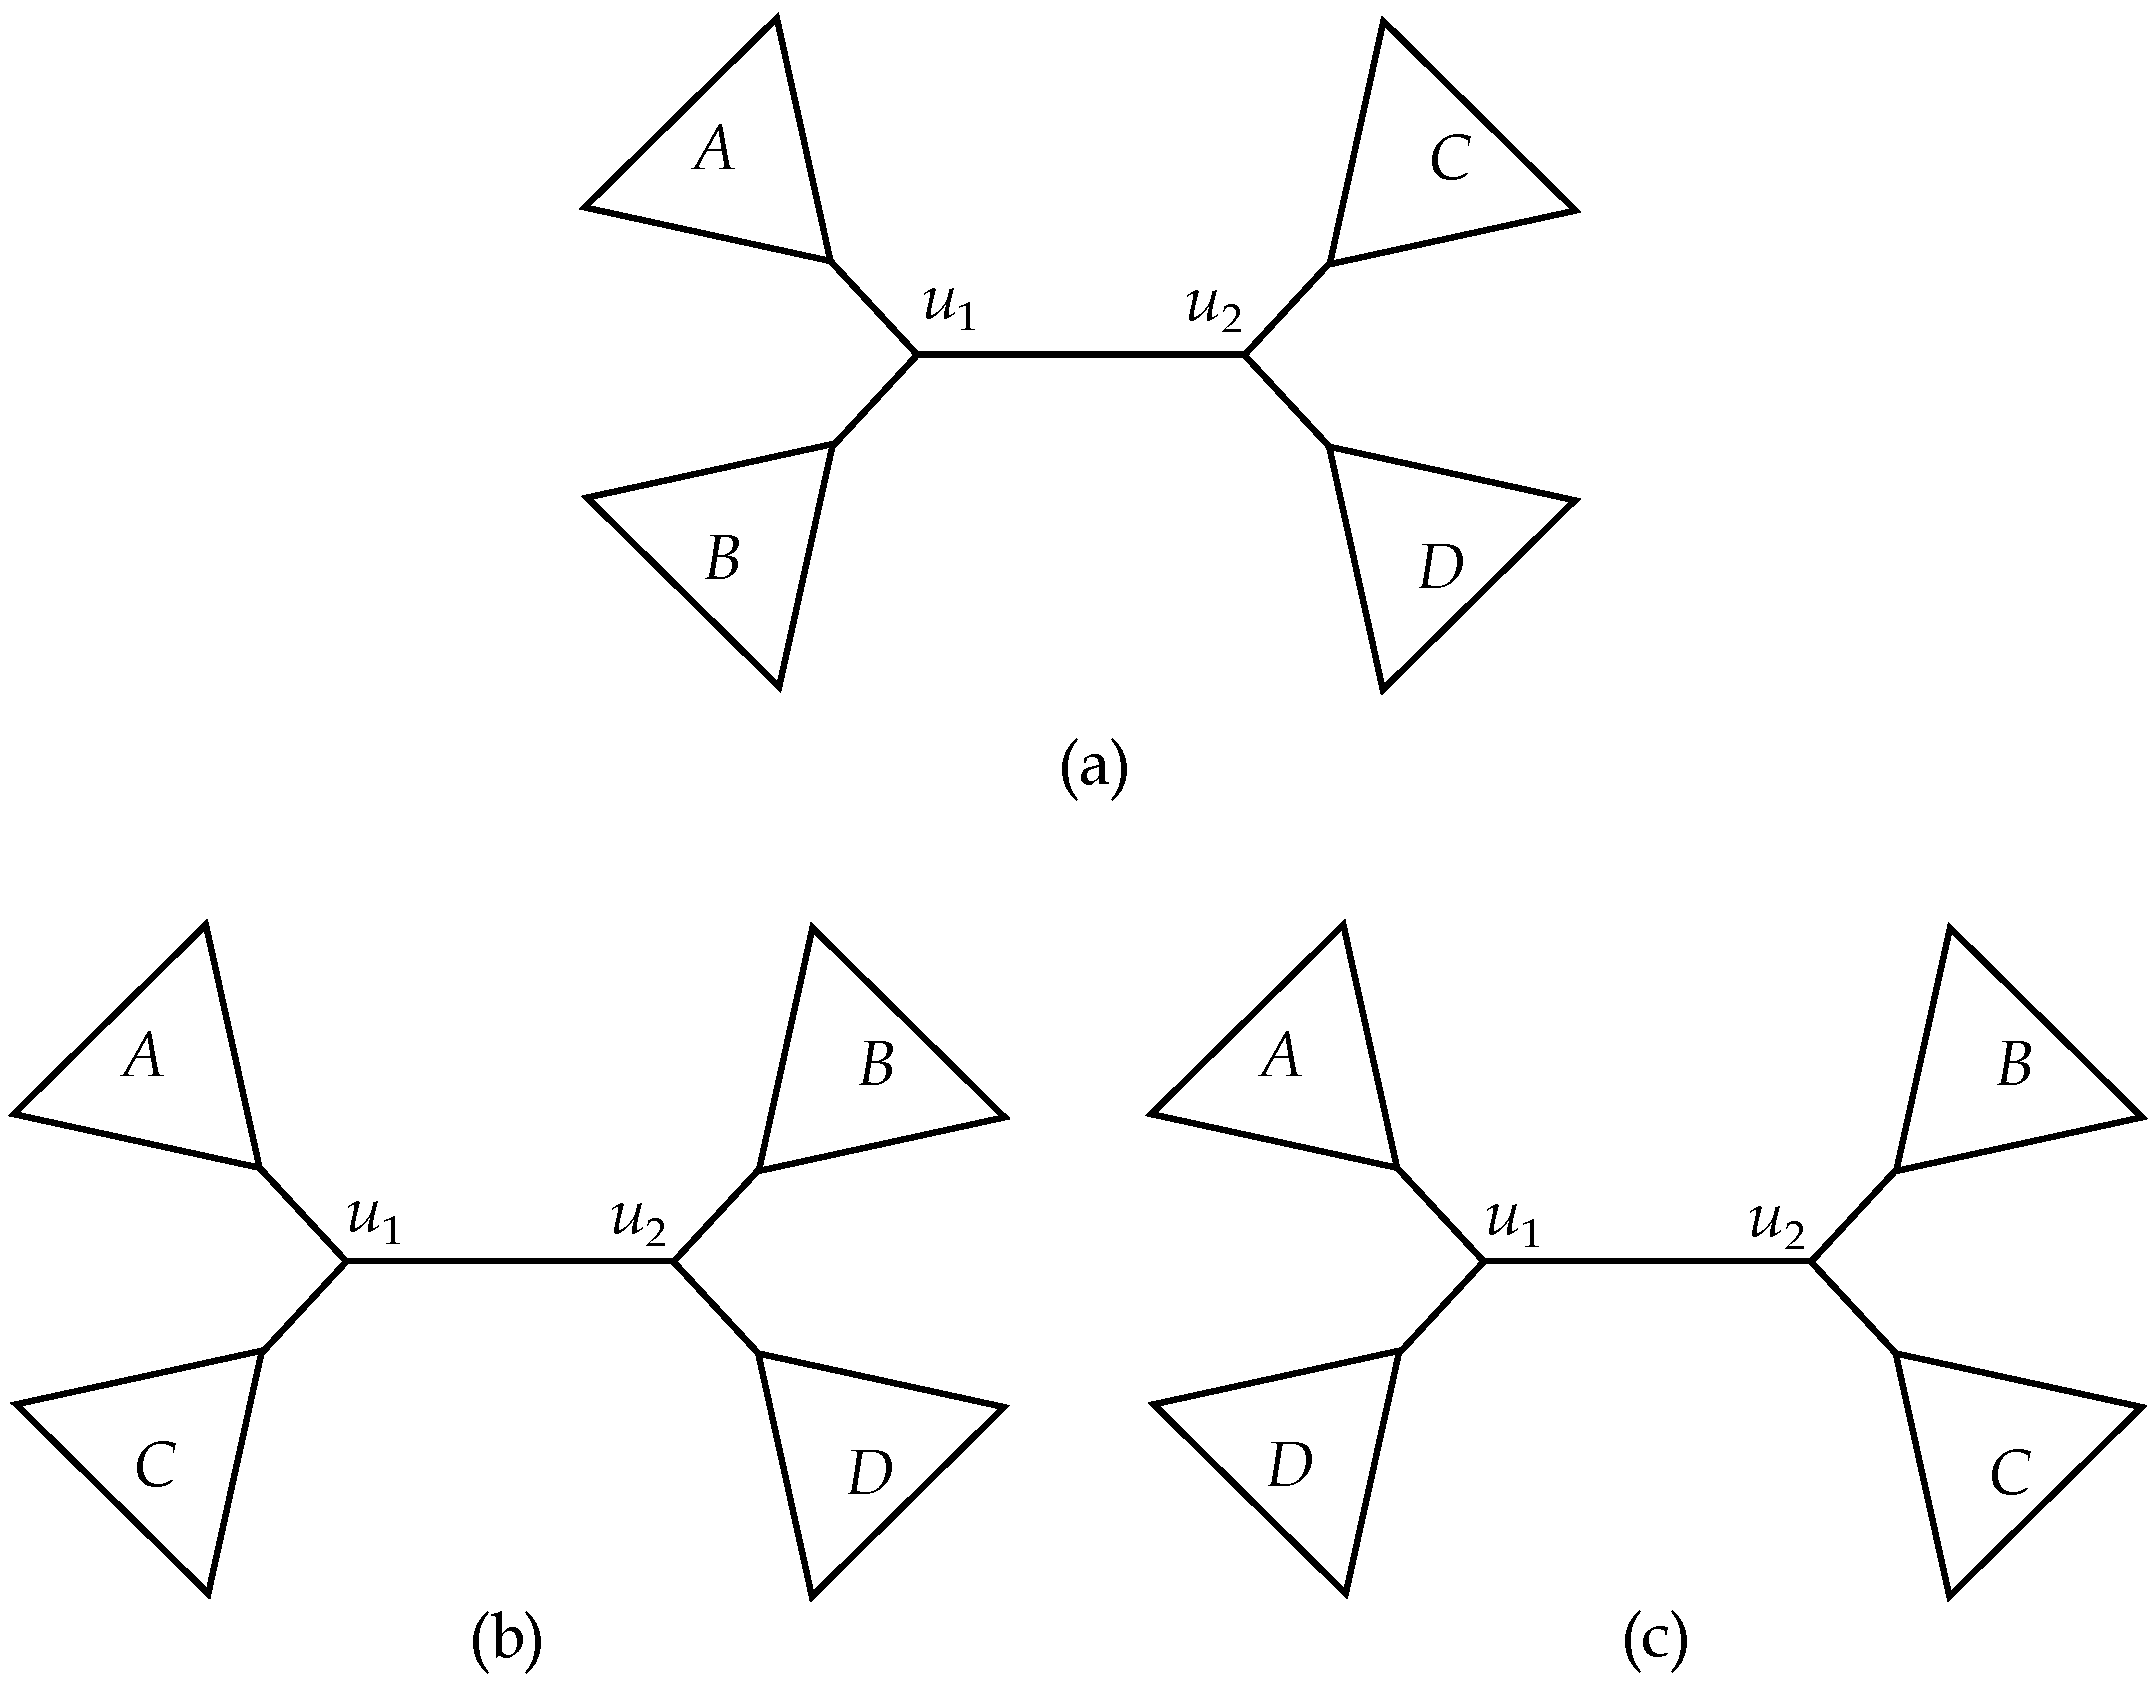
\includegraphics[width=0.7\linewidth]{Figure3.pdf}
        \caption{\label{fig:fig1}\textbf{Nearest Neighbor Interchange (NNI) move on an internal edge.} (a)
A species tree ST , and (b)-(c) the neighbors of ST resulting from one NNI move on edge
e = (u1 , u2 ). A, B, C, and D are the sets of taxa in the four subtrees around edge e.
}   
    \end{figure}
    
    \subsection{Figures}
    We intend to put Figure \ref{fig:fig1} at the top of a page.
    
    \subsection{Mathematical Equations}
    Let $n_1|n_2|n3$ be a tipartition defined on an internal node u of a binary tree T. The number of tripartitions mapped to u is given by Eqn. 1.
    
    \begin{equation} \label{eq1}
        \begin{split}
        \mathcal{NQ}(n_1, n_2, n_3) & = 
            \begin{pmatrix}
                    n_1 \\
                    2
                \end{pmatrix}
                \begin{pmatrix}
                    n_2 \\
                    1
                \end{pmatrix}
                \begin{pmatrix}
                    n_3 \\
                    1
                \end{pmatrix}
                +
                \begin{pmatrix}
                    n_2 \\
                    2
                \end{pmatrix}
                \begin{pmatrix}
                    n_1 \\
                    1
                \end{pmatrix}
                \begin{pmatrix}
                    n_3 \\
                    1
                \end{pmatrix}
                +
                \begin{pmatrix}
                    n_3 \\
                    2
                \end{pmatrix}
                \begin{pmatrix}
                    n_1 \\
                    1
                \end{pmatrix}
                \begin{pmatrix}
                    n_2 \\
                    1
                \end{pmatrix} \\
        & = \frac{n_1 n_2 n_3 (n_1 + n_2 + n_3 - 3)}{2} \\
        \newline
        \end{split}
    \end{equation}

    \section{Conclusions}
    The major objectives of this assignment are listed below (please do not ignore the font sizes).
    \begin{itemize}
     \item{\Huge{To see if students have adequately practiced different aspects of writing in \LaTeX.}} \pagebreak
     \item{\LARGE{To assess the ability of the students in preparing manuscripts in \LaTeX.}}
     \item{{To see if the students can add various basic components (e.g tables, figures, equations) to a \LaTeX manuscript.}}
     \item{To see if the students can leverage the available materials (both offline and online) to do something which has not explicitly been in the class.}
    \end{itemize}
\end{document}
